\section{Introduction}
\label{sec:intro}

The problem of double-degenerate mergers is one that has been well-studied numerically, statistically and observationally.  Since there is a well-defined parameter space of possible white dwarf (WD) and brown dwarf (BD) binary systems, it is relatively easy to categorize all possible merger types.  In this report, we will survey the observational characteristics and statistics of double-degenerate mergers.  We will classify these mergers according to the chemical composition of the more massive of the mergering WDs and BDs.

\subsection{Population Statistics}
\label{ssec:populationstatistics}

\begin{figure}
\centerline{\includegraphics[width=1.1\hsize]{wdbinarymasses.pdf}}
\caption{Plot of mass ratio ranges for WD binaries of various compositions.  Compositions were assumed to map uniquely onto mass via: He = 0.15 - 0.45 {\Msun}, CO = 0.45 - 1.1 {\Msun}, and ONe = 1.1 - 1.4 {\Msun}.  These values should be taken as guidelines, and not strict delinations between chemical compositions.  The curves are lines of constant gravitational wave chirp mass for inspiralling binaries.  The shaded region contains all CO WD binaries whose total mass is equal to or exceeds {\Mchan}, and are therefore expected to cause SNe Ia (see Sec. \ref{sec:withcarbon-oxygencompanions} for details.  From \cite{mars11}, their Fig. 1.}
\label{wdbinarymasses}
\end{figure}

WD mass and composition are both dependent on the evolutionary path of the WD progenitor star. A 0.15 - 0.45 {\Msun} WD will have a core comprised mostly of helium, a 0.45 - 1.1 {\Msun} WD will have a core of carbon and oxygen, and a 1.1 - 1.4 {\Msun} WD will have an oxygen-neon-magnesium core \citep{loreig09,mars11}.  (Work has been done, however, to show that these ranges are not set in stone; eg. \cite{moros09}.)  Brown dwarfs have masses of $\sim 0.08$ {\Msun} or lower \citep{stamw08}.

%A brown dwarf is a degenerate object composed largely of hydrogen, having never achieved the pressures and temperatures necessary for stable hydrogen burning.  While obviously formed from a very different stellar evolution channel, like WDs they are nonrelativistic degenerate bodies, and so obey the same stability arguments that have been detailed in the previous sections for white dwarfs.  Mergers between brown dwarfs, and between brown and white dwarfs, should be within the realm of physical possibility.

Close-in WD binaries are the result of common envelope evolution earlier in the binary's history.  Gravitational radiation or magnetic braking then drives the binary into a semi-detached state \citep{motl+07,nele+01}.  It is estimated that there are on order of $10^7$ - $10^8$ such semi-detached systems in the Milky Way alone \citep{motl+07,nele+01,mars11}.  Therefore any transients created by mass transfer within such systems should be frequently observed.

Statistically, mergers of certain types of WD binaries from Fig. \ref{wdbinarymasses} will dominate over others.  According to \cite{tremblay}, the mass distribution of DA white dwarfs (which comprise the vast majority of WDs) is narrowly peaked around $M = 0.65$ \Msun.  This suggests that the majority of WD binary interactions will be between near equal-mass CO WD pairs.  Binary evolution, however, will skew the population statistics of binary constituents.  \footnote{For example, in almost all cases a main-sequence binary system will undergo two stages of mass transfer to create a double degenerate system (one for the giant phase of each star).  The first phase of mass transfer must not result in common-envelope evolution; this requires a near-unity mass ratio between the two MS stars (see \cite{vkercj10} for details).  The most likely merger, then, is between two WDs of similar mass.}  \cite{han98} uses Monte Carlo simulations of binary evolution to determine that the birth rate of close-in WD binaries in the Milky Way is $\sim 3 \times 10^{-2}$ yr$^{-1}$, with 63\% being He-CO WD binaries, $\sim$ 2\% He-He, and 35\% CO-CO.  \citeauthor{han98} also gives merger rates: $5.7 \times 10^{-3}$ yr$^{-1}$ for He-He, $1.81 \times 10^{-2}$ yr$^{-1}$ for He-CO and $5.7 \times 10^{-3}$ yr$^{-1}$ for CO-CO mergers.  \cite{nele+01a}'s population sythesis models give different values for birth rates: a total rate of $4.8 \times 10^{-2}$ yr$^{-1}$, with 53\% of the binaries containing two He WDs, 25\% containing two CO WDs (including hybrid CO WDs with thick He envelopes), 20\% containing a CO and an He WD, and $\sim 1$\% containing ONeMg WDs.  The total merger rate for WDs of all sorts is $2.2 \times 10^{-2}$ yr$^{-1}$.  The differences between the two studies can be attributed to different common envelope inspiral efficiencies and treatments of mass transfer and stellar evolution.  (Each author also had multiple models with different treatments of such factors as star formation, WD cooling, etc.)

The frequency of BD-BD and BD-WD mergers has not been, to the best of our knowledge, quantified.

\subsection{Stability of Mass Transfer}
\label{ssec:stabilityofmasstransfer}

Another factor to consider is the stability of mass transfer between the binary constituents - if mass transfer is stable, then no merger will occur.  Stability depends critically on the mass ratio $q = M_2/M_1$ between the donor star ($M_2$) and the accretor star ($M_1$), and whether or not spin and orbital angular momentum can be efficiently coupled to each other.  We sketch a simple argument for stability in this section.  \cite{marsns04} has performed more detailed analysis of binary stability, and give more accurate stability criteria in agreement with the argument made here.

We first consider the case in which some process, for example tides or magnetic induction, is able to return spin angular momentum to orbital angular momentum, thus helping to stabilize mass transfer, meaning that (on the timescales of the merger) $\dot{J}_{orb} = 0$.  The orbital angular momentum of a binary system is $J_{orb} = (M_1M_2/M)\sqrt{GMa}$, where $M = M_1 + M_2$ and $a$ is the orbital separation.  From this we may derive $\dot{J}_{orb}/J_{orb} = \dot{M}_1/M_1 + \dot{M}_2/M_2 - \dot{M}/2M + \dot{a}/2a$.  We shall assume conservative mass transfer (this is backed by the simulations in Sec. \ref{ssec:mechanicsofwdmergers}, which show less than 1\% of stellar material becomes unbound even by extremely super-Eddington mass transfer), meaning $\dot{M}_1 = -\dot{M}_2$.  Putting this together gives us

\begin{equation}
\dot{J}_{orb}/J_{orb} = 2(q - 1)\frac{\dot{M}_2}{M_2} - \frac{\dot{a}}{a},
\label{adotovera}
\end{equation}

\noindent noting that $\dot{J}_{orb}/J_{orb} = 0$.  We use Paczynski's estimate for the Roche lobe of $M_2$, $R_L \approx 0.46a(M_2/M)^{1/3}$, valid for $q$ $\lesssim$ 1 \citep{eggl83}.  Differentiating and using Eqn. \ref{adotovera}, we obtain

\begin{equation}
\frac{\dot{R}_L}{R_L} = 2(q - \frac{5}{6})\frac{\dot{M}_2}{M_2}.
\label{rochedotoverroche}
\end{equation}

If we estimate a WD equation of state as a polytrope with $n = 3/2$, we obtain a mass-radius relation \citep{motl+07} \footnote{Note this is an equilibrium mass-radius relationship, which may not be a good approximation for a WD undergoing mass transfer.  See \cite{loreig09} for an semi-analytical treatment that takes this into account.}

\begin{equation}
R \propto M^{-1/3}.
\label{massradiusrelation}
\end{equation}

\noindent Assuming the constant of proportionality is the same for all WD equations of state, this indicates the less massive white dwarf overflows its Roche lobe first during any mass transfer, validating the use of Eqn. \ref{rochedotoverroche} (as all mass transfer will have $q$ $\lesssim$ 1)  \citep{came09}.  This results in the WD losing mass and expanding further per Eqn. \ref{massradiusrelation}.  The counteracting effect is increase in binary orbital separation due to the fact that the lower-mass WD is the donor star (Eqn. \ref{adotovera}).  We can take the derivative of Eqn. \ref{massradiusrelation} to obtain for the donor star $\dot{R}_2/R_2 = -\dot{M}_2/3M_2$.  Comparing this expression to Eqn. \ref{rochedotoverroche}, and requiring that $R_2$ expands more slowly than $R_L$, we obtain the following criterion for stability:

\begin{equation}
2(q - \frac{5}{6}) < - \frac{1}{3} \rightarrow q < \frac{2}{3}.
\label{qcrit}
\end{equation}

If spin and orbital angular momentum coupling is negligible, a similar analysis can be peformed, using total angular momentum $J = J_{orb} + J_{spin} = (M_1M_2/M)\sqrt{GMa} + J_{spin}$, from which we may derive $\dot{J}/J_{orb} = \dot{M}_1/M_1 + \dot{M}_2/M_2 - \dot{M}/2M + \dot{a}/2a + \dot{J}_{spin}/J_{orb}$ \citep{marsns04}.  Following \citeauthor{marsns04} and \citeauthor{nele+01}, we assume only the spin of the accretor matters for the equation, and follow \cite{verbr88}'s representation of the spin-up of the accretor from direct impact accretion with $\dot{J}_{spin} = -\sqrt{GM_1R_h}\dot{M}_2$ ($\dot{M}_2$ is negative).  $R_h$ is the effective radius of the matter transferred onto the accretor, and is given by a fitting formula: $R_h = a(0.0883 - 0.04858\log({q}) + 0.11489{\log}^2(q) + 0.020475{\log}^3(q))$, valid for all plausible WD binary mass ratios \citep{verbr88}.  Dividing this by $J_{orb}$ to obtain $\dot{J}_{spin}/J_{orb} = -\sqrt{(1 + q)r_h}\dot{M}_2/M_2$, we recognize that conservative mass transfer ($\dot{J} = 0$), and obtain \citep{marsns04,nele+01}

\begin{equation}
\frac{\dot{a}}{a} = 2(q - 1 + \sqrt{(1 + q)r_h})\frac{\dot{M}_2}{M_2},
\label{adotovera2}
\end{equation}

\noindent where $r_h = R_h/a$.  Using the same argument that gave us Eqn. \ref{qcrit}, we may obtain a new stability criterion \citep{nele+01,verbr88}

\begin{equation}
2(q - \frac{5}{6} + \sqrt{(1 + q)r_h}) < - \frac{1}{3} \rightarrow q \lesssim 0.219.
\label{qcrit2}
\end{equation}

\begin{figure}
\centerline{\includegraphics[width=0.8\hsize]{stabilityfig.pdf}}
\caption{Stability of mass transfer parameterized by the masses of the donor and accretor WDs.  The ``always unstable'' region follows from Ineq. \ref{qcrit}, and the ``disk accretion''/``definitely stable'' region is below Ineq. \ref{qcrit2} (Ineq. \ref{qcrit2} is not plotted, but falls roughly near the sub-Eddington/super-Eddington boundary).  The stability criterion for the middle region should fall between Ineqs. \ref{qcrit} and \ref{qcrit2}.  \citeauthor{hanw99} and \citeauthor{marsns04} both consider all super-Eddington accretion systems to result in merger, while \citeauthor{gokhpf07} suggest that accretion that is intially super-Eddington may eventually stabilize.  SPH simulation conducted by \citeauthor{dan+11} was performed for mass ratios indicated by squares and labels - all these systems merged, though P1 and P2 required several tens of orbits before doing so.  From \cite{dan+11}, their Fig. 1.}
\label{stabilityfig}
\end{figure}

\noindent Fig \ref{stabilityfig} from \cite{dan+11} summarizes this, indicating the zone of guaranteed instability given by Ineq. \ref{qcrit}, and the boundary between direct impact accretion and disk accretion (calculated from \cite{nele+01}).  Disk accretion results in good coupling between orbital and spin angular momenta, and since the region falls below Ineq. \ref{qcrit}, it is definitely stable.  (See section 4.5 of \citeauthor{marsns04}, however, for evidence that disk accretion does not stabilize mass transfer at all; the fact that disk accretion systems are stable would then be largely due to Ineq. \ref{qcrit2}.)  This leaves a large region of direct impact accretion in the middle of the two stability regions that may or may not be stable - if no coupling returns spin angular momentum to orbital angular momentum, most of the region should be unstable, as given by Ineq. \ref{qcrit2}.  \cite{marsns04} find that the stability in the middle region is dependent primarily on the synchronization timescale of the binary system, a conclusion supported by \cite{gokhpf07}'s stability analysis\footnote{Another fact that needs to be considered is that even in unstable mass transfer, if the donor can survive long enough for $q$ to drop to a value conducive to stable mass transfer, ultimately the system does not merge \citep{gokhpf07}}.  Unfortunately tidal interaction in WD binaries is not well understood (see Sec. \ref{ssec:synchronization}).

A number of numerical studies have been performed to explore mass ratios of uncertain mass transfer stability, and the results have not been conclusive \citep{mars11}.  For example, \cite{motl+07} used a (grid-based) self-consistent field method to determine that for an initial mass ratio $q_{init} = 0.4$ there is enough spin-orbit momentum coupling to ensure stability.  On the other hand SPH simulations by \cite{dan+11} using the Helmholtz equation of state yielded a merger for $q = 0.4$, and have shown unstable mass transfer for binaries down to $q = 0.25$.  \citeauthor{dan+11} also show that for such mergers a careful construction of the initial conditions results in a long period of mass transfer (several tens of orbital periods) before full disruption of the donor, suggesting that their results can be compatible with the results from \citep{motl+07}.  For the purposes of this paper, we will consider an extreme mass ratio merger to be a plausible (if rare, given WD mass distribution statistics) occurence.

DOES DAN USE SYNCHRONIZED BINARIES???  PAPER DOESN'T SAY - E-MAIL DIRECTLY.

It should be noted that \cite{dan+11} also show that merger simulations are sensitive to initial conditions, and point out that the approximate initial conditions of other simulation groups such as \citeauthor{loreig09}, \citeauthor{guerig04} and \cite{pakm+10} may distort their findings.  This not only applies to merger stability and merger timescales, but also central temperatures of post-merger remnants.

\subsection{Synchronization}
\label{ssec:synchronization}

Estimates of the synchronization timescale in binary systems give $\tau_{S} \sim 10^{12}$ yr from radiative damping, and $\tau_{S} \sim 10^{15}$ yr from viscosity \citep{marsns04}.  To compare, the timescale for angular momentum loss from gravitational wave radiation is \citep{segrcm97}

\begin{equation}
\tau_{\mathrm{grav}} = 5 \times 10^5 \left( \frac{a}{10^5 \mathrm{km}}\right)^4 \frac{M_{\odot}}{M_1} \frac{M_{\odot}}{M_2} \frac{M_{\odot}}{M_1 + M_2} \mathrm{ yr}.
\label{gravtimescale}
\end{equation}

\noindent In the latter stages of evolution, this value is around $\tau_{S} \sim 10^{6}$ yr.  It is then likely that neither donor nor accretor are synchronized at the time of merger\footnote{A close-in WD binary should merger within $10^8$ to $10^9$ yrs after formation \cite{segrcm97}.  Of course, any transients caused by mergers seen today must have occured within this time!}.  Turbulent viscosity and non-radial mode excitation, on the other hand, can potentially have $\tau_{S} << 500$ yr, and even small magnetic fields, properly oriented, can significantly enhance viscosity \citep{marsns04,ibentf98}.  Also, the viscous timescale scales as $a^6$, while Eqn. \ref{gravtimescale} scales as $a^4$; this indicates that should viscosity ever synchronize a WD binary, this binary will be synchronized for the remainder of its inspiral \citep{ibentf98}.  Whether or not a binary will be synchronized is still largely an unsolved problem \citep{mars11}.

If we were to suppose a WD system could synchronize, then viscous dissipation should heat up both WDs significantly.  \cite{ibentf98} perform long equal-mass binary evolution calculations that assumes the binary system is synchronized, and the rate of tidal heating is equal to the rate of spin kinetic energy increase. (SO DOES IT SAP ROTATION????)  They find that over the course of the last $10^4$ yrs before merger heating from synchronization can increase the temperature of a 1.0 {\Msun} (with a 1.0 {\Msun} companion) by an order of magnitude.  While most of the thermal energy that is radiated away during this heat-up is in the form of neutrinos, the EM luminosity increases by almost five orders of magnitude.  At the time of merger, each 1.0 {\Msun} WD would shine with $\sim 100$ L$_{\odot}$ and have a temperature of $\sim 10^8$ K, making the system a significant X-ray source.  The luminosity just before merger increases with WD mass, and the period of time over which luminosity increase occurs drops with WD mass: a 0.3 {\Msun} with an equal-mass companion will increase in luminosity by two orders of magnitude over $10^6$ yr.  If the efficiency by which rotational energy is converted to thermal energy is reduced to 10\% the maximum efficiency in the 1.0-1.0 {\Msun} binary, the final luminosity drops by a factor of about 1000.  In all cases simulated, \citeauthor{ibentf98} found temperatures were insufficient to ignite nuclear fusion.  The periods of increased luminosity are all in the range of $10^2 - 10^6$ years, which, while short compared to the liftime of the binary, are far too long to be considered transients.

\subsection{Super-Eddington Mass Transfer}
\label{ssec:super-eddingtonmasstransfer}

The luminosity of the accretion flow is set by the amount of energy liberated from transfering $M_2$'s mass from the inner Lagrange point to the surface of the accreting star.  Therefore, $L_{acc} = \dot{M}_2(\phi_{L1} - \phi_{R1})$  \citep{hanw99}.  For many values of $q$, however, mass transfer will be higher than the Eddington mass transfer limit.  \citeauthor{hanw99} analytically investigated super-Eddington accretion between compact object, and concluded that under these conditions, the luminosity is truncated at the Eddington luminosity of $L_{Edd} = 4{\pi}GM_1m_pc/\sigma_T$, where $\sigma_T$ is the Thomson scattering cross-section, while the rest of the energy either goes into mass ejection or is retained as thermal energy.  They further find that often less than 50\% of the mass of the accretion stream is ejected from the system.

The Eddington mass accretion rate can be estimated by equating $L_{acc}$ with $2L_{Edd}$ (where the factor of 2 takes into account two proton masses for every free electron, as is appropriate for fully-ionized He or CO) to obtain \cite{marsns04}

\begin{equation}
\dot{M}_{Edd} = \frac{8{\pi}GM_1m_pc}{\sigma_T(\phi_{L1} - \phi_{R1})}.
\label{eddingtonmassacc}
\end{equation}

\noindent Steady-state mass transfer rates, assuming perfect coupling between spin and orbit angular momentum, can be determined by equating $\dot{R}_2/R_2 = \dot{R}_L/R_L$, and using Eqns. \ref{adotovera} and \ref{rochedotoverroche} to obtain

\begin{equation}
\dot{M}_{acc} = M_2\frac{\dot{J}_{orb}/J_{orb}}{2/3 - q}.
\label{ssmassacc}
\end{equation}

\noindent The value of $\dot{J}$ can be assumed to be $\dot{J}_{GR} = -(32/5)(G^3/c^5)(M_1M_2M/a^4)J_{orb}$ due to gravitational wave emission ($J_{orb}$ was defined in Sec. \ref{ssec:stabilityofmasstransfer}).  Equating Eqns. \ref{eddingtonmassacc} and \ref{ssmassacc} can be used to estimate the sub-Eddington/super-Eddington mass accretion rate transition in Fig. \ref{stabilityfig} (see more accurate estimates in eg. \citeauthor{gokhpf07}).

The thermal energy retained by the WD causes the outer envelope to expand, resulting in the creation of a common envelope that leads to runaway mass transfer and a merger \citep{hanw99}.  This expectation is used in all the stability studies cited in this paper, though it has not been conclusively proven \citep{motl+07,marsns04,gokhpf07}.

The light curve of a merger would consist of a combination of the Eddington luminosity, convolved with effects from radius expansion, and cooling of the ejected mass, which can be estimated via Arnett's method.  This is done in Sec. \ref{ssec:lightcurveestimation}.

\subsection{Mechanics of WD Mergers}
\label{ssec:mechanicsofwdmergers}

\cite{guerig04}, \cite{yoonpr07} and \cite{loreig09} performed a sampling of high-resolution ($\sim 4 \times 10^5$ particle) SPH simulations of WD mergers.  In all three works, the binaries are assumed to be non-synchronized, per \citeauthor{segrcm97}.  Earlier simulation work on such mergers were marred by issues of excess artificial viscosity, which more modern studies have attempted to rectify by using more complex prescriptions of viscosity.  In particular, \citeauthor{guerig04} uses a Balsara switch (which they noted may have been insufficient), \citeauthor{yoonpr07} an adaptive viscosity method and Balsara switch, and \citeauthor{loreig09} a method based off of Reimann-solvers plus a switch.  Table \ref{simtable} summarizes their results.

\begin{table}
\centering
\caption{Table of WD merger simulation results from \cite{guerig04}, \cite{loreig09}, \cite{yoonpr07} and \cite{pakm+10}.  M$_{bin}$ is the binary system total mass, written as a sum of the binary's constituent masses, M$_{rem}$ is the mass of the merger remnant, M$_{disk}$ the Keplerian disk, and M$_{ej}$ ejected mass, all of which are in units of {\Msun}.  The mass-composition relationships given in Sec. \ref{ssec:populationstatistics} are used for all runs.  T$_\mathrm{mmax}$ is the maximum temperature achieved during the merger, while T$_\mathrm{rem}$ is the maximum temperature of the remnant.  \citeauthor{guerig04} only gives final remnant temperatures in a few cases.  Note that because \citeauthor{guerig04} only used a Balsara switch, and did not use equal-mass SPH particles in their runs, which will lead to artificially high viscosities and numerical artifacts \cite{loreig09}.  Between the three runs, it is consistently shown that nuclear burning is negligible for CO-CO mergers, while \citeauthor{loreig09} found significant non-explosive nuclear processing for He-CO and CO-ONeMg mergers.}
\begin{tabular}{cccccccc}
\hline & \\[-1em]\hline
Group & M$_{bin}$ & M$_{rem}$ & M$_{disk}$ & M$_{ej}$ & T$_\mathrm{max}$ (K) & T$_\mathrm{rem}$ (K) & E$_\mathrm{nuc}$ (ergs)\\
\hline & \\[-1em]\hline
\citeauthor{loreig09}	& 0.3+0.5	& 0.62 & 0.18 & $10^{-3}$ & $6 \times 10^{8}$ & $6 \times 10^{8}$ & $1 \times 10^{42}$ \\
	& 0.4+0.8	& 0.92 & 0.28 & $10^{-3}$ & $6.5 \times 10^{8}$ & $6 \times 10^{8}$ & $1 \times 10^{44}$ \\
	& 0.6+0.6	& 1.10 & 0.10 & $10^{-3}$ & $6.3 \times 10^{8}$ & $6.2 \times 10^{8}$ & 0 \\
	& 0.6+0.8	& 1.10 & 0.30 & $10^{-3}$ & $1.6 \times 10^{9}$ & $8.7 \times 10^{8}$ & $1 \times 10^{41}$ \\
	& 0.6+1.2	& 1.50 & 0.30 & $10^{-3}$ & $1.0 \times 10^{10}$ & $1.0 \times 10^{9}$ & $2 \times 10^{44}$ \\
\hline
\citeauthor{yoonpr07}	& 0.6+0.9 & 1.10 & 0.40 & & $1.7 \times 10^{9}$ & $5.6 \times 10^{8}$ & $1 \times 10^{45}$ \\
\hline
\citeauthor{guerig04}	& 0.4+0.4	& & & 0 & $2.2 \times 10^8$ & $1.6 \times 10^8$ & \\
	& 0.4+0.6	& & & $3.32 \times 10^{-3}$ & $7 \times 10^{9}$ & & \\
	& 0.4+1.2	& & & $3.54 \times 10^{-2}$ & $3.1 \times 10^9$ & & \\
	& 0.6+0.8	& & & $2.82 \times 10^{-3}$ & $1.4 \times 10^9$ & $5 \times 10^8$ & \\
	& 0.6+1.0	& & & $6.48 \times 10^{-3}$ & $1.6 \times 10^9$ & & \\
	& 0.8+1.0	& & & $6.52 \times 10^{-3}$ & $2.0 \times 10^9$ & & \\
\hline
\cite{pakm+10}	& 0.89+0.89	& & & $2.9 \times 10^9$ & & \\
\hline
\hline & \\[-1em]\hline
\end{tabular}
\label{simtable}
\end{table}

%-The mass values derived from \citeauthor{yoonpr07}'s run assume all of the 0.9 {\Msun} primary and 33\% of the 0.6 {\Msun} secodary form the remnant.  IS THIS ASSUMPTION BAD????

In general the mergers simulated all finish within several orbital periods - this is in contrast to the simulations done by \citeauthor{motl+07} and \citeauthor{dan+11}, and is likely due to a choice of initial conditions.  When the two WDs begin the merger process, the less massive WD fills its Roche lobe and begins to transfer mass (as expected), is completely disrupted tidally, and eventually forms an outer envelope and a fat disk around the more massive WD (due to highly super-Eddington accretion, most of the material is not incorporated into the larger WD).  During this time temperatures often reach $10^{11}$ K at the point of contact between the accretion stream and the more massive WD, initiating nuclear reactions, but they are quickly quenched as this region expands, loses degeneracy, and cools.  \citeauthor{loreig09} notes the expanding material then redistributes itself over the surface of the more massive WD, forming a ``hot corona''.  \citeauthor{loreig09} and \citeauthor{yoonpr07} both find rigidly rotating cores, differentially rotating outer remnant layers (spun up by the merger) and sub-Keplerian disk, while \citeauthor{guerig04} finds a completely rigidly rotating remnant (likely due to just using a Balsara switch).  \citeauthor{loreig09} also perform a 0.6-0.6 {\Msun} CO WD equal mass merger, and \citeauthor{guerig04} perform a 0.4-0.4 {\Msun} He WD merger, with both observing noticable differences from unequal mass mergers.  No real ``disk'' is formed, though the merger remnant has an extended ellipsoidal shape, and the peak temperature is near the centre of the remnant instead in the hot corona.  Additionally, the entire remnant rigidly rotates.  In all simulations presented, very little ($< 10^{-3}$ {\Msun}) mass is ejected from the system.

Nuclear burning in the merger simulations produces energies ranging from $10^{42}$ to $10^{45}$ ergs, and \citeauthor{loreig09} note $10^{21}$ to $10^{37}$ ergs are emitted as neutrinos (a strong function of merger mass), and $10^{39}$ to $10^{41}$ ergs are emitted as gravitational waves.  As the amount of ejected mass is minimal, photon emission should roughly be Eddington luminosity limited, and therefore is also orders of magnitude below the nuclear burning.  Nuclear processing is significant for He-CO and CO-ONeMg mergers, while CO-CO mergers have little nuclear processing \citep{loreig09}.

\cite{pakm+10} perform an 0.89-0.89 merger simulation, which qualitatively agrees with the equal mass mergers of \citeauthor{loreig09} and \citeauthor{guerig04}, and track the hottest points in the system during merger.  They find that a detonation should arise from a hotspot with density $3.8 \times 10^6$ g/cm$^3$ and temperature $2.9 \times 10^9$ K, resulting in the complete disruption of the system.  See Sec. \ref{sec:withcarbon-oxygencompanions} for details.

\begin{figure}
\centerline{\includegraphics[width=0.6\hsize]{mergerfig.png}}
\caption{xy and xz plane plots of the merger between a 0.6 and a 0.8 {\Msun} CO WD at different times.  Colours indicate different temperatures.  The creation of a hot corona is quite evident in the xz plane plot.  From \cite{loreig09}, their Fig. 2.}
\label{mergerfig}
\end{figure}

\citeauthor{loreig09} also find some particles ejected into highly eccentric orbits, and expect them to emit high-energy photons when colliding with and becoming absorbed into the sub-Keplerian disk.  They obtain a light curve for this phenomenon by following a similar calculation for neutron star and black hole merger remnants by \cite{ross07}.  The calculation assumes that highly eccentric particles impacting the disk lose all their kinetic energy, and that all this energy is turned into high-energy photons - the light curves should therefore be taken as (extreme) upper limits to the shape of the curve.  The transient has a peak luminosity upper limit of $\sim 10^{51}$ erg, but only lasts for several hundred seconds to several tens of hours.  Nevertheless, \citeauthor{loreig09} find large luminosities for a wide range of merger mass ratios, and state this would be a tell-tale signature of a WD binary merger.  See Fig. \ref{fallbackacc} for light curves.

\begin{figure}
\centerline{\includegraphics[width=0.8\hsize]{fallbackacc.png}}
\caption{Plot of bolometric luminosity versus time for high-eccentricity material falling onto the Keplerian disk.  These plots set upper limits to the luminosity over time (real values may be orders of magnitude lower).  From \cite{loreig09}, their Fig. 8.}
\label{fallbackacc}
\end{figure}

\subsection{A Merger Light Curve Estimation}
\label{ssec:lightcurveestimation}

Using Arnett's light curve prescription, we can estimate the light curve formed by a merger.  Luminosity will come from two sources: the cooling of ejected material and the Eddington-luminosity remnant.  We therefore assume either $\sim 10^{-3}$ {\Msun} or $\sim 2 \times 10^{-2}$ {\Msun} of non-radioactive ejecta with input energy from an Eddington-luminosity remnant, the mass of which is varied.  Ejecta velocity is assumed to be the escape velocity.  Ejecta composition (important for recombination) is in accordance with those stated for Fig. \ref{wdbinarymasses}.  For He, we use a recombination energy of 24.6 eV and a recombination temperature of $10^4$ K.  For CO, we follow Arnett's estimate of simply using 13.6 eV and 7500 K.

The result is a very weak transient whose luminosity is often just the assumed Eddington luminosity of the central remnant (obviously, this luminosity will decrease over time as accretion ceases; this decline is not modelled), with a maximum peak caused solely by liberated photons during recombination.  Fast recombination is assumed in this experiment - slow recombination might give different peak values and rise times.

\begin{figure}
\centerline{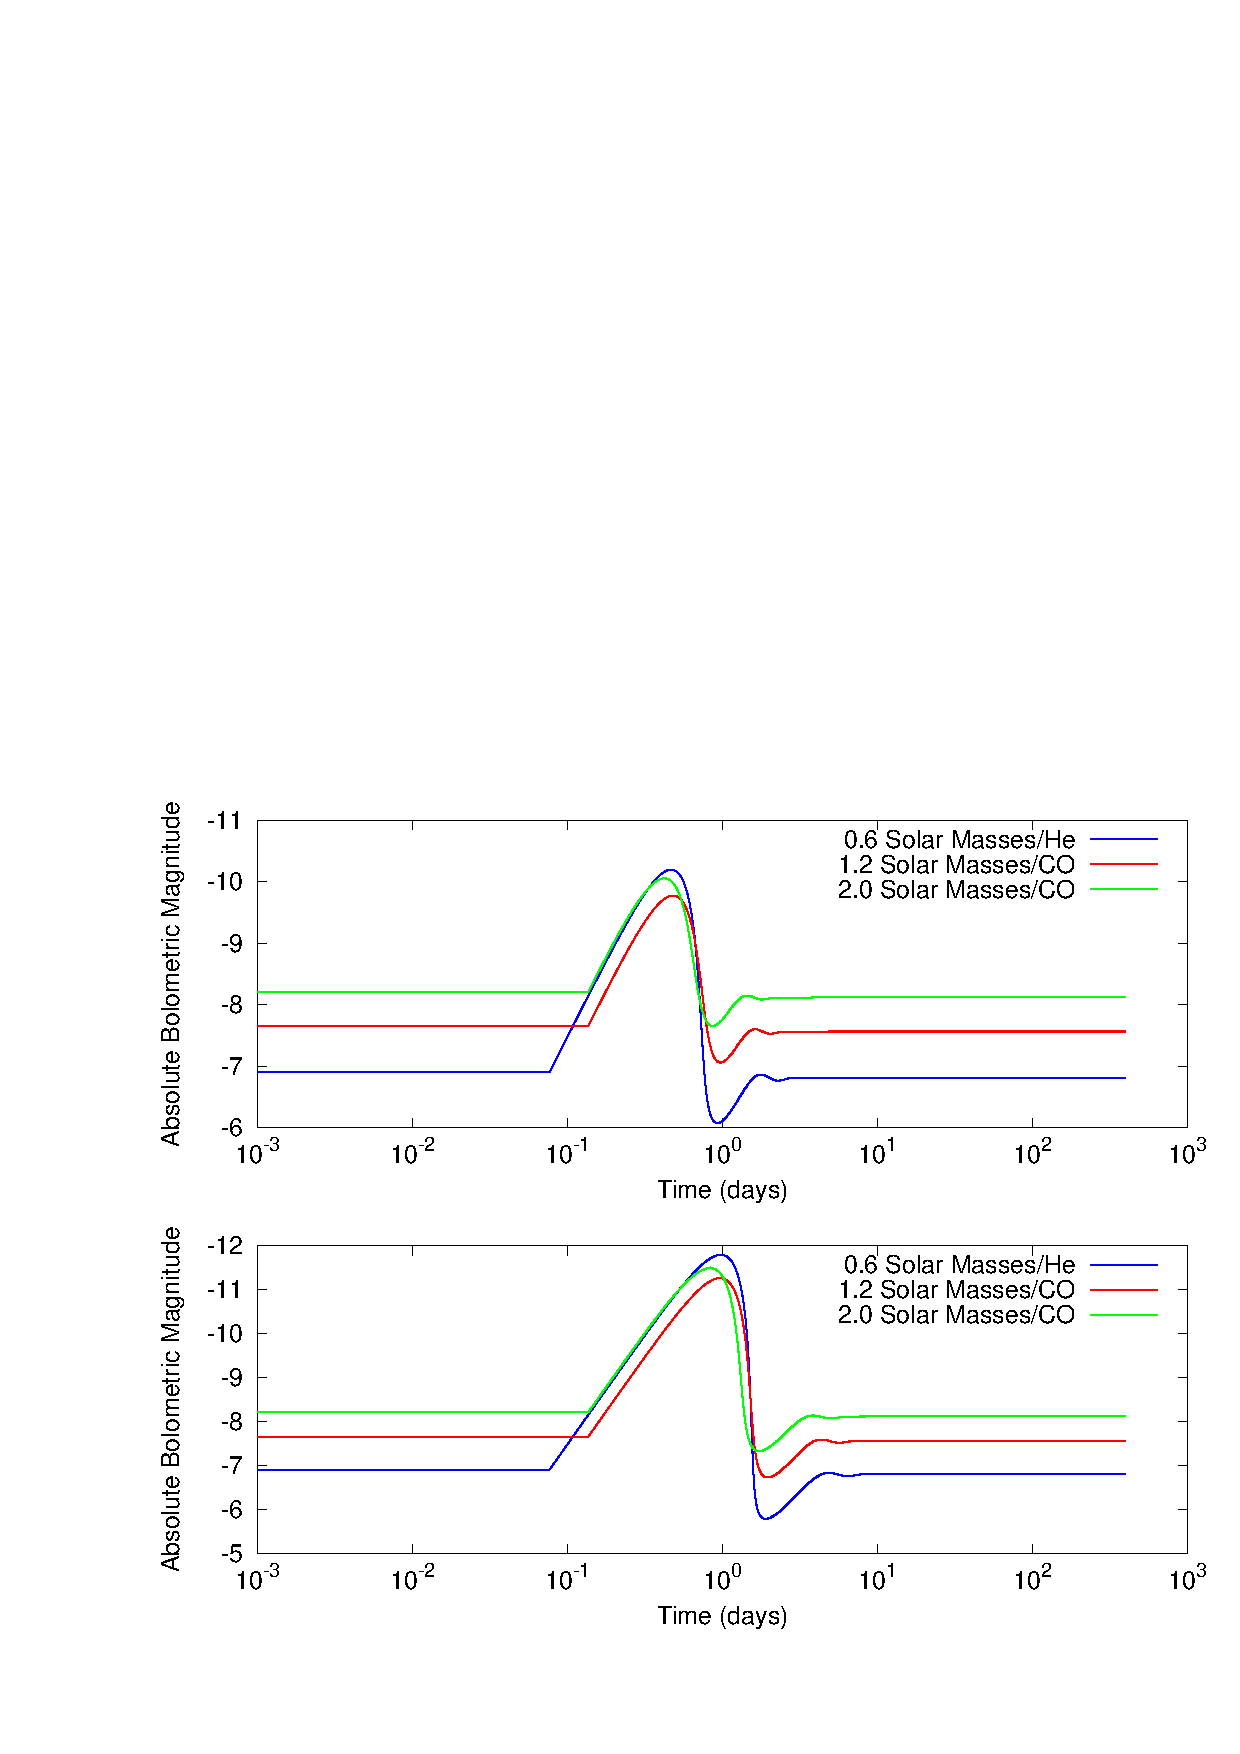
\includegraphics[width=1.0\hsize]{pathetictransient.pdf}}
\caption{Bolometric light curves vs. time calculated using an implementation of Arnett's semi-empirical explosion model.  Absolute magnitudes were calculated with Vega as M = 0.  The top figure assumes $10^{-3}$ {\Msun} of He or CO ejecta travelling at escape velocity from a 0.6 {\Msun} He, 1.2 {\Msun} CO or 2.0 {\Msun} CO remnant (remnant and ejecta have the same composition).  The bottom figure assumes $10^{-2}$ {\Msun} of ejecta.  Peak light for $10^{-3}$ {\Msun} is $\sim$ -10 mag at $\sim$ 0.5 days.  Peak light for $10^{-2}$ {\Msun} is $\sim$ -11.5 mag after $\sim$ 1 day.}
\label{pathetictransient}
\end{figure}

It has been found, then, that in general mergers themselves do not (except in the cases of \cite{pakm+10} and the eccentric material fallback transient \cite{loreig09}) produce appreciable transients.  It is still an open question whether, post-merger, the accretion of the hot disk onto the remnant core will result in a transient.  We now explore this possibility.